\vspace{.08in}
\noindent \textbf{Fast ROMs for Turbulence.} (Task 2.)
The goal of this task is to push the state-of-the-art for ROM-based 
simulation of turbulent flows.
The equations of interest are the incompressible Navier-Stokes equations
(NSE) with energy transport,
\begin{eqnarray} \label{eq:ns}
&&
\partial_t \bu \,+\, \bu \cdot \nabla \bu \,-\, \frac{1}{Re} \nabla^2 \bu
\,+\, \nabla p \;=\; \bff, \hspace*{.4in} \nabla \cdot \bu \;=\; 0, 
\\ \label{eq:therm} 
&&
\partial_t T   \,+\, \bu \cdot \nabla T   \,-\, \frac{1}{Pr\,Re} \nabla^2 T
\;=\; q, 
\end{eqnarray}
subject to appropriate boundary and initial conditions. Here, $Re$ and $Pr$ are
respective Reynolds and Prandtl numbers, $q$ is the volumetric heating, and
$\bff$ is a body force that may be temperature dependent.
   To simplify the exposition, we here consider only the NSE (\ref{eq:ns}).

One of the distinguishing features of turbulent flows is that, because of
sensitivity to initial conditions, they are repeatable only in a statistical
sense.  There is no hope of repeating the exact trajectory of the solution in a
turbulent flow between two experiments or two simulation algorithms.  ROMs,
therefore, must target {\em space-} and/or {\em time-averaged} QOIs such as
velocity profiles,  turbulent-kinetic energy distributions, and Nusselt
numbers.  For the same reason, such quantities are also the currency of
engineering design and thus reasonable measures of the success of a ROM as a
low-cost analysis tool.  Thus, the {\em objective} of this project is
prediction of engineering QOIs, rather than prediction of precise 
trajectories.  This simplified objective is one of the key features that makes
the problem tractable.

    While our focus will be on mean engineering quantities, we note that the
time-evolving ROMs {\em also} provide reasonable surrogates for unsteady
behavior (or they would not be good predictors of the mean) and therefore can
be used to visualize flows, which is often useful for engineering insight
(e.g., identifying stagnant and ejected vortices).  We also propose to augment
qualitative visual analysis of the unsteady behavior with quantitative
monitoring of the amplitudes, frequencies, and gradients of QOIs at specified
locations in subsets of the domain, which will help assess potential
thermal striping, thermal fatigue, and thermal stratification effects.

The ROM for the Navier-Stokes equations starts with a collection of $K$
snapshots, $\bu^k(\bx) := \bu(\bx,t^k) \in X_0^{\cN}$, corresponding to
numerical solutions of the Nek5000/RS full-order model (FOM) at well-separated
timepoints.  For any $\bu \in X_0^{\cN} \subset \cH^1_0$ we have a
corresponding vector of basis coefficients $\buu=[\bu_1\dots \bu_{\cN}]^T$ such
that $\bu(\bx)=\sum_{j=1}^\cN \bu_j \phi_j(\bx)$, with $\phi_j(\bx)$ the
underlying spectral element basis functions spanning the FOM approximation
space, $X_0^\cN$.  We collect the snapshots into the a matrix $\bU_K = [ \buu^1
\dots \buu^K ]$.  From these, one forms the Gramian, $\bU \in \cR^{K \times K}$
with $\bU_{k,k'} := (\bu^k,\bu^{k'})_A$, where $(\cdot,\cdot)_A$ is the energy
($\cH_0^1$) norm.  Following standard POD methodology, the basis functions $\{
\uzeta_n \}$ for the ROM derive from the first $N$ eigenmodes of $\bU$,
\\[-3.3ex]
\begin{eqnarray} \label{eq:eig}
\bU\uz_k&=&\lambda_k \uz_k,\;\;\;\uz_k \in \RR^K, \;\;\; \lambda_1 
        \ge \cdots \ge \lambda_K \ge 0
                    \\[1.2ex] \label{eq:podbasis}
\uzeta_n &:=& \bU_K \uz_n, \;\;\; n\,=\,1,\dots,N \, < \, K.
%                    \hspace*{1.1in} \mbox{\em POD basis set.} 
\end{eqnarray}

Defining $\bzeta_n(\bx) := \sum_{j=1}^{\cN} (\uzeta_n)^{}_j \phi_j(\bx)$, 
the standard POD Galerkin formulation follows by inserting the reduced-basis
expansion
\\[-6.5ex]
\begin{eqnarray} \nonumber
\tbu(x,t) &=& \sum_{n=1}^N \, \bzeta_n(\bx) a_n(t)  \\[-3.3ex] \nonumber
\end{eqnarray}
into the Galerkin statement for the NSE, resulting in the following
evolution equation for the reduced-order basis coefficients, $a_n(t)$:
{\em For each $i=1,\dots,N$,} \\[-3.3ex]
\begin{eqnarray} \label{eq:erom}
\sum_{j=1}^N M_{ij} \dd{a_j}{t} &=&
- \, \sum_{k=1}^N \, \sum_{j=1}^N C_{ijk} a_k(t) a_j(t) 
\,-\, \frac{1}{Re} \sum_{j=1}^N A_{ij} a_j(t),
\end{eqnarray}
where 
$M_{ij} := \int \bzeta_i \cdot \bzeta_j  \, d\bx$ is the mass matrix,
$C_{ijk} := \int \bzeta_i \cdot ( \bzeta_k \cdot \nabla \bzeta_j) \, d\bx$
is the nonlinear interaction term and 
$A_{ij} := \int \nabla \bzeta_i \cdot \nabla \bzeta_j \, d\bx$
is the viscous term.  We note that, in the case of fixed geometries, 
the divergence and pressure terms drop out of (\ref{eq:erom}) because
the underlying basis is already divergence free.
   A semi-implicit formulation for (\ref{eq:erom}) leads to an $N \times N$
linear system of the form,
\begin{eqnarray} \label{eq:eromd}
E(\ua^l,Re) \ua^{l+1} &=& \uft (\ua^l,Re),
\end{eqnarray}
for each timestep $t^l$ (using a larger timestep size than the FOM).

For typical turbulence problems, the standard approach is to use
$K$$\approx$1000 high-fidelity solution snapshots (i.e., full
velocity/temperature fields) to form $N$$\approx$20--200 basis functions
through POD or some other low-rank approximation approach.  For relatively
small $N$ ($<100$), the low-dimensional ODE (\ref{eq:eromd}) can be advanced
extremely fast---\textbf{in just a few minutes on a laptop it is possible to
evolve tens-of-thousands of convective time units,} much longer than feasible
with a FOM, even on an exascale platform, which is one of the reasons that ROMs
are interesting for long-time transients.  Moreover, it is relatively easy to
adjust equation parameters to have a nominal pMOR tool.

There are, however, several challenges to bringing the preceding scenario to fruition.
The first is to ensure that the ROM can accurately track the quantities
of interest (QOIs) produced by the FOM, even at the same parameter point.
Accuracy is by no means assured, particularly for turbulent flows
where energy is dissipated by small-scale structures that are generally absent
from POD bases.  Several stabilization strategies are possible, such as Leray
regularization, in which the advecting field is smoothed \cite{wang2012proper}, 
or constrained evolution, in which each basis coefficient is constrained
to the range observed in the projection of the snapshot space onto the bases. 
\cite{fick18}.  Alternative approaches include modification of the approximation
space.  For example \cite{akkari19} uses a decomposition of modes
into distinct sets minimizing the $L^2$ error (for accuracy) and the $\cH^1$
error (for stability).  In \cite{khodkar2019}, a basis is derived from Green's
functions approximations.

   Under prior NEUP support, Kaneko \cite{kaneko22a,kaneko22} developed an
augmented-basis method (ABM) wherein a set of standard POD basis functions,
$\{\bzeta_i(\bx) \}$,  is augmented with a subset of their nonlinear
interaction terms, $\{\bzeta_i \cdot \nabla \bzeta_j\}$.  The success of the
ABM is illustrated in the turbulent pipe flow examples of Fig. \ref{fig:abm},
which shows that standard POD Galerkin and Leray regularization can converge at
lower Reynolds numbers $Re$ with a sufficient number of basis functions, $N$,
but that the required number of basis functions rapidly increases with $Re$.
Given the $O(N^3)$ costs for the ROM, these methods are limited to relatively
low $Re$.  The ABM and the constrained approaches, however, perform much better
because of their stability.  The ROM accuracy for the turbulent kinetic energy 
and thermal QOIs is similar to that of the  mean velocity seen in Fig. \ref{fig:abm},
but the ABM can be overly dissipative at higher $Re$.  \textbf{Understanding the
mechanism for this anomalous behavior is an objective of the proposed work,}
which we will explore through extensive unit tests such as minimal-channel
flows, thermal striping in a T-junction, etc.
  One possible solution, suggested by Akkari {\em et al.} \cite{akkari19} is to
choose $N=N_P + N_d$ modes with the decomposition of the number
of POD modes, $N_P$, and dissipative modes (here, ABM), $N_d$ based on
readily available energy estimates.  
Kaneko \cite{kaneko22a,kaneko22} demonstrates that the ABM indeed serves as an
energy sink, precisely as required for stability.
  Following \cite{wang2012proper,mou2021}, we can also consider filter-based
stabilization as is commonly used for LES of turbulent flows.  We are 
presently pursuing this question in a collaboration with Iliescu at V. Tech.

\begin{figure}[t] \centering
{\setlength{\unitlength}{1.0in} \begin{picture}(6.5,1.40)(0,0.05)
 \put(-.08,0.15){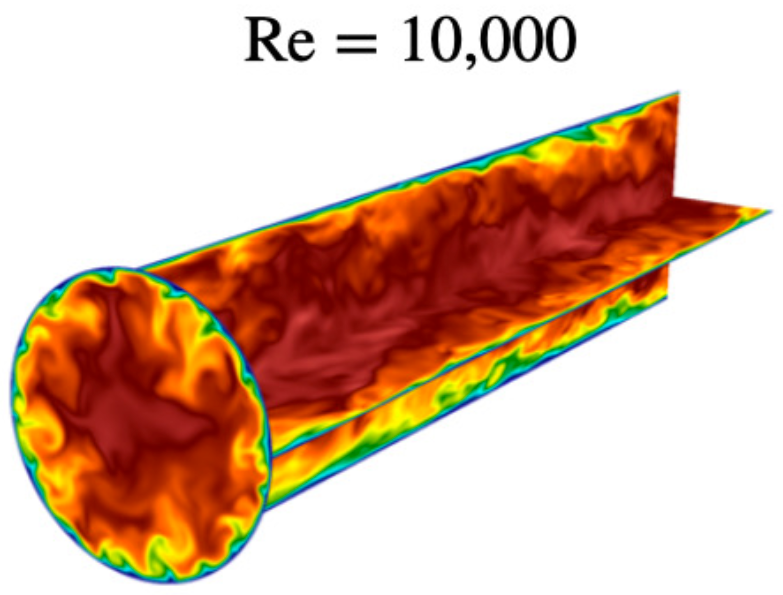
\includegraphics[width = 0.24\textwidth]{figs/kaneko_diss_pipe_r10k.png}}
 \put(1.75,0.00){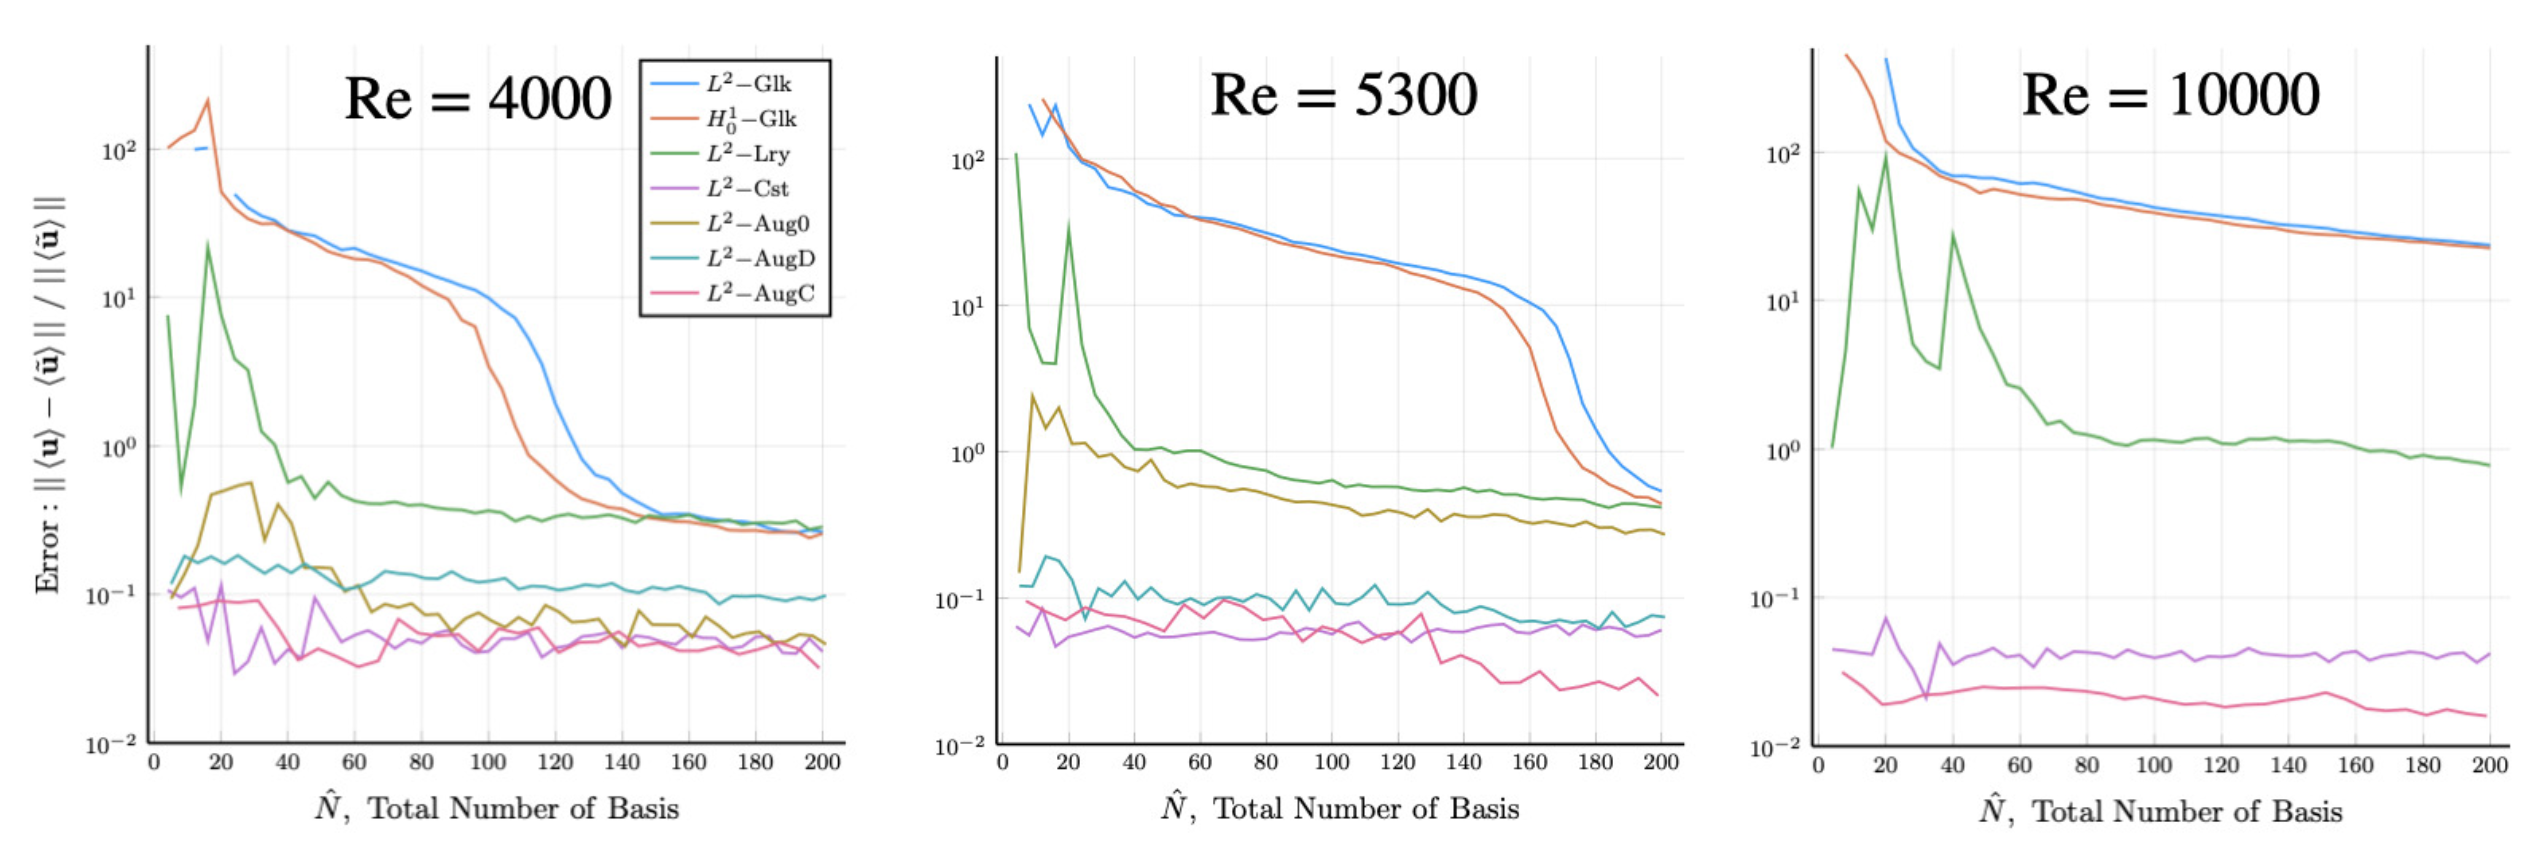
\includegraphics[width = 0.70\textwidth]{figs/kaneko_diss_pipe_ubar.png}}
\end{picture}}
\caption{
\textbf{(left)} Nek5000 DNS of turbulent pipe flow at $Re_D$=10,000;
\textbf{(right)} Mean velocity error in ROM reproduction results for Galerkin POD 
    ($L^2$-Glk, $H^1$-Glk), Leray- and constrainted-based regularization 
    ($L^2$-Lry, $H^1$-Cst), and ABM with three different subsets of the nonlinear terms
    ($L^2$-Aug0=$\bzeta_0 \cdot \nabla \bzeta_j+ \bzeta_j \cdot \nabla \bzeta_0$,
    $L^2$-AugD=$\bzeta_j \cdot \nabla \bzeta_j$,
    $L^2$-AugC=$L^2$-Aug0 $\bigcup$ $L^2$-AugD) \cite{kaneko22a,kaneko22}.
\label{fig:abm}}
\end{figure}

Stability is a requirement for a successful ROM, but it does not guarantee
accuracy of all (or any) of the QOIs.  The standard numerical approach to
improving accuracy is to increase $N$, which can be seen to be beneficial for
the less performant ROMs of Fig. \ref{fig:abm}.  For $Re=4000$, there is a
significant error reduction for the Galerkin ROMs as $N$ is increased from 100
to 140.  For $Re=5300$, the transition occurs for $N=140$ to 180.  For
$N=10,000$, we cannot observe a transition for $N \leq 200$, but one might
speculate that it could be found if we take $N$ large enough.  Unfortunately,
each step of (\ref{eq:eromd}) requires a contraction with the 3rd-order tensor
$C_{ijk}$, which requires $O(N^3)$ operations and dominates the cost of the
online (and, potentially, the offline) portion of the ROM.  Mitigation of this
leading-order cost is of primary importance and we address several strategies
to this end below.  Possibilities include replacing the nonlinear term
with an approximation based on the discrete empirical interpolation method
(DEIM) \cite{deim2010} or replacing the rank-3 tensor $C_{ijk}$ with
the sum of $R$ rank-1 tensors, which reduces the $O(N^3)$ cost to $O(NR)$.
Even if $R=N$, this reduction affords considerable savings, which implies
that one could enrich the approximation space with substantial increases in $N$.
(An important technical detail for stability, being explored by UIUC Ph.D.
student Ping-Hsuan Tsai, is to ensure that the low-rank tensor inherits the
skew-symmetry properties that are intrinsic to advection operators in
closed systems.)


A equally significant concern is that (\ref{eq:eromd}) can deviate substantially
from the projection of the modes onto the FOM due to the presence of potentially
spurious attractors that are an artifact of truncation, typically manifest as
energy pile-up in the high wavenumber modes \cite{fick18,rempfer00} or a
result of (unavoidable) lack-of-repeatability in cases where the flow 
exhibits spatio-temporal chaos.  Recommendations on how to detect the latter
are presented in \cite{tsai22a}.  

For the former, the unstable behavior relates to the well-known closure problem
in LES and other turbulence-modeling scenarios where the smoothness of the
approximating modes $\{\bzeta_n\}$ prevents generation of adequate dissipation
(through $Re^{-1} (\bzeta_j,\bzeta_j)_A$ ) unless the corresponding
coefficients have large amplitude.  
Several stabilization strategies are possible, such as Leray regularization
\cite{wang2012proper} or constrained coefficient evolution
\cite{fick18,kaneko20a}.  Alternative approaches include modification of the
approximation space.  For example \cite{akkari19} uses a decomposition of modes
into distinct sets minimizing the $L^2$ error (for accuracy) and the $\cH^1$
error (for stability).  In \cite{khodkar2019}, a basis is derived from Green's
functions approximations.
   Under prior NEUP support, Kaneko \cite{kaneko22a,kaneko22} developed an
augmented-basis method (ABM) wherein a set of standard POD basis functions,
$\{\bzeta_i(\bx) \}$,  is augmented with a subset of their nonlinear interaction
terms, $\{\bzeta_i \cdot \nabla \bzeta_j\}$.
  The success of the ABM is illustrated in the turbulent pipe flow
examples of Fig. \ref{fig:abm}, which shows that standard POD Galerkin and
Leray regularization can converge at lower Reynolds numbers $Re$ with a
sufficient number of basis functions, $N$, but that the required number of
basis functions rapidly increases with $Re$.  Given the $O(N^3)$ costs for the
ROM, these methods are limited to relatively low $Re$.  The ABM and
the constrained approaches, however, perform much better because of their
stability.  The turbulent kinetic energy behavior is similar to the
mean velocities shown in Fig. \ref{fig:abm}, but the ABM
can be overly dissipative at higher $Re$.  The mechanism for this anomalous
behavior is under investigation.



%  Rather than trying to explicitly add dissipation, as considered by
%  some authors \cite{lumley88}, we follow the novel formulation in \cite{fick18},
%  in which the equality (\ref{eq:eromd}) is replaced by the constrained
%  minimization problem, \\[-3ex]
%  \begin{eqnarray} \label{eq:const}
%  \ua^{l+1} &=& \mbox{argmin}_{\ua \in \RR^N} || E^l \ua - \uft^l ||_2^2
%  \;\;\;\;\mbox{s.t.} \;\; \alpha_n \, \leq \, a_n \, \leq \, \beta_n,\;\;\; n=1,\dots,N,
%  \end{eqnarray}
%  where the constraints are derived from the observation snapshot set, $\bU_K$.
%  For each $\bzeta_n$, one computes $\alpha_n = \min_k (\bzeta_n,\bu^k)^{}_A$ and
%  $\beta_n = \max_k (\bzeta_n , \bu^k)^{}_A$.  (In practice, each window 
%  $[\alpha_n,\beta_n]$ is increased a few percentage points.)  

%    We remark that (\ref{eq:const}) defaults to the Galerkin POD when the
%  constraints are inactive.  However, as shown in \cite{fick18}, because
%  they keep the coefficients within observed bounds, the constraints tend to
%  make (\ref{eq:erom}) stable {\em and} more accurate for lower values of $N$
%  than required by the standard Galerkin POD, which leads to considerable cost
%  savings in the overall analysis process.  

%  This constrained approach makes dual use of the snapshot data.  First, in
%  formulating the optimal approximation set and, second, in developing the
%  constraint bounds.   All computational effort in identifying 
%  $\{\uzeta_n,\, \alpha_n,\, \beta_n \}$ is at the scale of the FOM, which
%  implies that these operations need to be embedded in the parallel
%  (offline) solver.  A major objective of this project is to effect a 
%  tight integration of the offline procedure (\ref{eq:eig})--(\ref{eq:const})
%  into Nek5000/RS that will be easy to use.

%%%   
%%%   \vspace*{.1in}
%%%   \subsubsection*{Parametric Problem}
%%%   The objective of {\em parametric} model order reduction ($p$MOR) is to use the
%%%   evolution equation (\ref{eq:erom}) with a {\em different} parameter $\up^* \in
%%%   \cP$.  (Here, we take the example of (\ref{eq:erom}), where the parameter is
%%%   $Re$, but one can design ROMs to support additional free parameters.
%%%   Exploration of the technical details of such a process will be central to the
%%%   project.)  As a first guess, one could simply set $Re=Re^*$ in (\ref{eq:erom})
%%%   and run the ROM in the online (fast) mode to evaluate the desired QOIs at
%%%   $\up^*  (=Re^*)$.  Such an approach, however, would not give any confidence
%%%   regarding the quality of the result.  In order to be useful, dual-norm-based
%%%   error indicators have been developed to provide scaled estimates of the
%%%   error in the QOI at any point $Re^* \neq Re$.  These error indicators are used
%%%   in two ways.  
%%%   
%%%   First, in a {\em training mode}, one can evaluate the error in the existing ROM
%%%   at every point in $\cP_{\mbox{\tiny train}} \subset \cP$ to ensure that the error is
%%%   sufficiently small for all $\up \in \cP_{\mbox{\tiny train}}$.   If it is not,
%%%   construct an additional ROM (i.e., in the {\em offline mode}) at a new point
%%%   $\up' \in \cP_{\mbox{\tiny train}}$ that corresponds to the maximum estimated error
%%%   in the QOI and add this point to the set of anchor points, $\cP_{\mbox{\tiny anchor}}
%%%   \subset \cP_{\mbox{\tiny train}}$.  This {\em greedy} training algorithm, which
%%%   choose anchor points based on current error estimates, is repeated until the
%%%   error indicator (the minimum realized across all ROMs in the anchor
%%%   space) meets the desired tolerance for all points in $\cP_{\mbox{\tiny train}}$.
%%%   
%%%   Second, the error estimate plays a crucial role in reducing the costs
%%%   of the online evaluation and online/offline training phases. (Training, as
%%%   described above, involves several online evaluations coupled with a few offline
%%%   computations.)   When one has reduced basis sets $\{\uzeta_n\}$ from multiple
%%%   parameter points it is common to combine them into a larger approximation space
%%%   such that POD-Galerkin generates a projection onto this large space.  However,
%%%   with $O(N^3)$ complexity, such a large space is generally
%%%   impractical.  Moreover, for transitional flows, it makes little sense to mix
%%%   turbulent and laminar solution spaces.   A more effective strategy is to
%%%   estimate the QOI-error for each ROM associated with a point $\up' \in
%%%   \cP_{\mbox{\tiny anchor}}$ and choose the particular ROM that minimizes
%%%   the error indicator when evaluated at $\up^*$.
%%%   Thus, the error indicators allow one to down-select the approximation
%%%   space prior to evaluation of the ROM, with considerable cost savings.
%%%   (This strategy, in which the reduced bases are not mixed, is referred to
%%%   as an $h$-greedy strategy as convergence is realized through subdivision
%%%   of the parameter space.)
%%%   
%%%   %% {\em 
%%%   %% Do we mention the downside, that the convergence is only linear?
%%%   %% Is there any hope of remedying the linear convergence rate, a posteriori?}
%%%   
%%%   
%%%   \vspace*{.1in}
%%%   \subsubsection*{Key Developments}
%%%   
%%%   As noted in the Tasks, the principal extensions to the methodology of
%%%   \cite{fick18} include: extension to 3D; inclusion of thermal transport;
%%%   and addition of buoyancy, all coupled with extensive verification and
%%%   validation (V\&V) on NE-relevant problems.
%%%   
%%%      The extension to 3D is chosen as the first step because the mathematical
%%%   framework is unchanged between the 2D and 3D NSE.  The principal challenge will
%%%   be to ensure that the ROM accurately reproduces the desired QOIs for
%%%   thermal-hydraulics applications with a reasonable basis-set size, $N$.
%%%   %
%%%     For example,  \cite{merzari11b} reports that at least 200 modes are required
%%%   to capture 50\% of the energy for a counterflow T-junction at $Re=3500$.
%%%   Similarly, \cite{adrian10} find that $N\approx 250$ modes are required to
%%%   capture 50\% of the energy in the DNS of a turbulent boundary layer at
%%%   $Re_{\theta}=80$--1950.  
%%%       In the present context, the target problem choice of reproducing mean
%%%   quantities helps to reduce the required number of modes.
%%%       The constrained evolution (\ref{eq:const}) also assists in keeping the 
%%%   ROM closer to the underlying attractor of the FOM with fewer modes than would
%%%   otherwise be required \cite{fick18}.  
%%%      As an alternative to the hard constraints (\ref{eq:const}), we will 
%%%   explore the use of soft constraints such that the evolution will be smooth
%%%   in time.  This relaxation can be implemented by recasting the inequality
%%%   constraints as barrier functions with relatively wide barriers and solving 
%%%   the resultant unconstrained minimization problem.
%%%   
%%%      For a single ({\em reproduction}) ROM, the online $O(N^3)$ costs will
%%%   be relatively small compared to the $O(\cN)$ costs of the FOM.  The significant
%%%   increase in $\cN$ and potential increase in $N$, however, makes reduction of
%%%   the number of FOMs required for the pMOR essential.  The $h$-greedy training
%%%   strategy described above addresses this issue directly by
%%%   successively choosing anchor points where the error is largest.  If required,
%%%   we can pursue a more aggressive strategy in which the $h$-greedy algorithm adds
%%%   multiple points to $\cP_{\mbox{\tiny train}}$ for each training submission.
%%%   This approach significantly increases the amount of parallelism, which will
%%%   reduce training time and which is critically important for DOE's forthcoming
%%%   exascale architectures.
%%%   The size and complexity of the 3D offline problems necessitates seamless
%%%   integration with high-performance computing platforms.  Nek5000/RS already excels
%%%   in this respect, but developing an integrated framework that will automate the
%%%   process of running multiple FOMs will greatly simplify the overall analysis.
%%%      Additional acceleration strategies will include parallel evaluation of the
%%%   3rd-order tensor $C_{ijk}$, for which costs scale as $O(\cN N^3)$.
%%%      Because of the smoothness of the basis functions, $\{\bzeta_n(\bx) \}$, 
%%%   the $N^3$ entries in $C_{ijk}$ and other tensors can be most likely be
%%%   computed by integrating lower order spectral elements than required for the FOM.  
%%%   A preprocessing scan of the basis functions in this regard could be executed in
%%%   $O(N\cN)$ time to identify all spectral elements where reduction of the local
%%%   polynomial order, $o$, is feasible.  In 3D, the integration costs scale as
%%%   $O(o^3)$--$O(o^4)$, so slight reductions in order would yield significant
%%%   savings.
%%%   
%%%    Other possible work-reduction schemes include regional clipping, in which the
%%%   POD is derived from only a subset of the domain and which tends to reduce the
%%%   number of active modes \cite{merzari15a}.  In the proposed context, this
%%%   approach would result in unsteady boundary conditions that would need to be
%%%   appropriately addressed as extensions to current strategies for steady
%%%   inhomogeneous boundary conditions \cite{fick18}.
%%%      An alternative and complementary subdomain-POD approach has recently
%%%   been proposed in which DNS/LES is used only in the region of interest
%%%   and the ROM is used to drive the flow dynamics in the far-field region where
%%%   less detail might be required \cite{bergmann18}.  Such approaches are obviously
%%%   better suited to external aerodynamic flows rather than internal flows typical
%%%   of reactors, but might be applicable in large regions such as the upper plenum.  
%%%   
%%%   
%%%   The presence of thermal transport raises several additional considerations
%%%   in terms of strategy, costs, and implementation.   The minimization
%%%   problem requires a proper weighting of the NSE and energy equations, which
%%%   are readily derived from asymptotic/dimensional analysis.   In addition, the
%%%   error indicators will need to accommodate the thermal field, but they
%%%   are not more complex than those associated with the vector velocity
%%%   field \cite{fick18,patera05}.
%%%     For the thermal transport POD,
%%%     we view the bases $\{\bzeta_n\}$ as vector fields that include $d$
%%%   components of velocity plus temperature and then project these bases onto the
%%%   equation set (\ref{eq:ns})--(\ref{eq:therm}) to be evolved as a single
%%%   dynamical system.  This approach leads to complexity for the {\em online} 
%%%   model that is identical to the nonthermal case, save that the basis set may
%%%   need to be larger to adequately capture variance in $T(\bx,t)$.
%%%   
%%%    Additional complexities will arise if the properties are temperature
%%%   dependent.  If the dependency can be reasonably approximated 
%%%   by a linear model, then the complexity will amount to a modified
%%%   or perhaps additional 3rd-order tensor, such that the overall complexity
%%%   will remain at $O(N^3)$.
%%%     We note that the addition of buoyancy induces feedback from (\ref{eq:therm})
%%%   to (\ref{eq:ns}), but it is {\em linear} and therefore does not directly
%%%   contribute to the leading order complexity of the ROM aside from its
%%%   impact on the dynamics.   Exploration of these
%%%   dynamics is naturally one of the principal objectives of this project and we
%%%   will do so first through 2D problems and ultimately in full 3D configurations.
%%%   
%%%   We note that there is {\em another important use case} for the hydrodynamic ROM
%%%   when coupled with the energy equation.  Depending on the boundary conditions,
%%%   the thermal problem (\ref{eq:therm}) can take much longer to reach a
%%%   statistically steady state than the hydrodynamics (\ref{eq:ns}).
%%%   This disparity can arise, for example, if the channel is long with respect to
%%%   the hydraulic diameter or if the system has significant thermal mass such that
%%%   tens or hundreds of (long) flow-through times are required to reach thermal
%%%   equilibrium.  While the latter situation can often be mitigated by artificially
%%%   reducing the thermal inertia, the hydrodynamic ROM offers an alternative
%%%   solution to this thermal-hydraulics challenge.  Namely, one can run the
%%%   hydrodynamic ROM (\ref{eq:erom}), generate the corresponding velocity field,
%%%   and evolve the thermal solution without the need for the expensive velocity
%%%   and pressure updates.  We note that this {\em semi-reduced} model is
%%%   readily able to address thermal transients at costs that are significantly lower
%%%   than advancement of the FOM for the hydrodynamic problem. The stabilized
%%%   formulation (\ref{eq:const}) will ensure that the ROM reasonably tracks the
%%%   statistics of the FOM.  Moreover, in this {\em reproduction mode}, the velocity
%%%   and (possibly) the temperature field need not be resolved at their original
%%%   $O(\cN)$ fidelity, given that the basis functions $\bzeta(\bx)_n$ are smooth.
%%%   In Nek5000/RS, it's relatively simple to interpolate the basis functions onto
%%%   coarser meshes ($\cN_c < \cN$) by using a lower-order polynomial in the
%%%   underlying spectral element discretization or using Nek5000/RS's efficient (and
%%%   spectrally accurate) grid-to-grid interpolation.  Conversely, if one wanted
%%%   {\em higher} resolution for the thermal problem (e.g., in the case of high
%%%   Prandtl or Schmidt numbers), the reproduction could be evolved on a
%%%   higher-order spectral element mesh.
%%%   
%%%   \vspace*{.1in}
%%%   
